\documentclass[a4paper]{report}
\usepackage[top=30mm, bottom=30mm, left=30mm, right=30mm]{geometry}
\usepackage{times} % ???
\usepackage{graphicx} % for pictures
\usepackage{hyperref} % for internal links
\linespread{2}
\DeclareGraphicsExtensions{.jpg}
\usepackage[T1]{fontenc} % see http://tex.stackexchange.com/questions/664/

\begin{document}

\begin{abstract} % on the abstract page, we also need the title, my name, university of ..., graduation year
Nuclear Magnetic Resonance (NMR) spectroscopy is a technique for studying 
biological molecules such as proteins and metabolites at the atomic level.  
The information obtained from NMR is used to identify metabolites, identify 
binding partners, locate active sites and binding pockets, and obtain 
structural and dynamics information which can be used in drug design.  In 
order to study molecules using NMR, an NMR spectrometer is used to collect 
free-induction decay (FID) data sets from a pure, high-concentration sample 
of the molecule(s) of interest.  In subsequent analysis, the FID data is 
processed to frequency-domain spectra, which are then analysed to find peaks 
and assign the peaks to specific atoms in the molecule, in a process known as 
chemical shift assignment.  The typical process makes use of automated tools to 
speed up simple and tedious tasks where possible, but relies upon manual 
analysis for complicated and difficult cases.  Spectroscopists use a deductive 
strategy of iteratively applying previously identified rules to make analyses 
of specific cases.  Ambiguous cases are noted and deferred, or the highest 
probability interpretation is made.  Following chemical shift assignment, 
NOESY spectra are peak-picked and assigned, and finally a structure is 
calculated and refined.  During the analysis process, large amounts of data 
and metadata are generated.  However, much of this is not recorded and thus 
does not show up in archives such as the BMRB.  This raises serious 
reproducibility concerns, since the data and metadata describing how the 
analysis was carried out are lost.  Additional concerns include: how can 
practitioners successfully collaborate when data is missing?  How can errors 
be efficiently identified and corrected?  How can additional data be used to 
augment the analysis without having to restart the process from the beginning?  
The growing problems caused by irreproducibility in science have been noted 
recently.  The main contribution of this project is a definition of 
reproducibility within protein NMR, a strategy for rendering NMR analysis 
reproducible, a software implementation to enable reproducible analysis, a 
means for sharing reproducible data sets through a public archive; and a data 
set analysed using fully reproducible means.
\end{abstract}

\begin{titlepage}

Reproducible Protein NMR Data Analysis

Matthew Fenwick

B.S., University of Oklahoma, 2009

A Dissertation 
Submitted in Partial Fulfillment of the 
Requirements for the Degree of Doctor of Philosophy 
at the 
University of Connecticut 

2014
\end{titlepage}

% TODO optional copyright page
\pagenumbering{roman}
% TODO approval page
% TODO acknowledgements page

\tableofcontents

\listoftables

\listoffigures

\chapter{Introduction}
\pagenumbering{arabic}
\section{Protein NMR}
NMR (Nuclear Magnetic Resonance) spectroscopy is an experimental technique for 
studying proteins and other biological molecules at atomic resolution.  In 
comparison to other techniques for high-resolution characterization of 
biological molecules, NMR's significance as an experimental technique stems 
from its ability to collect detailed molecular data, from which further 
analysis can derive not only structural information but also dynamics, 
activity, and interactions with other molecules.  The importance of NMR 
spectroscopy to the structural biology community has steadily increased, as 
measured by the number of biologically relevant molecules that have been 
studied using the technique, and the corresponding data deposited into 
publicly available databases -- since 1990, the structures of nearly 9,000 
proteins that were solved using NMR have been deposited in the Protein Data 
Bank (PDB) \cite{pdb}, a facility for the archival and sharing of protein-related 
data, and NMR data is available for over 10,000 proteins in the BioMagnetic 
Resonance Bank (BMRB) \cite{bmrb}, a facility for the archival and sharing of 
specifically NMR-derived data.  The data collected using NMR techniques is 
important to the field of drug design, as it can aid in identifying potential 
binding partners based on surfaces as well as actual binding partners based on 
chemical shifts, and understanding biological processes.

In order to study proteins in solution using NMR, multi-step processes are 
employed to collect and analyze data.  An example process is described here 
as a series of independent stages.  Here is a brief outline of the example 
process, which will be expanded upon later:

\begin{itemize}
  \item data collection
  \begin{itemize}
     \item isolation and purification of sample of interest
     \item collection of time-domain data in an NMR spectrometer
  \end{itemize}
  \item spectral processing
  \begin{itemize}
     \item processing of time-domain data to frequency-domain spectra
  \end{itemize}
  \item spectral analysis
  \begin{itemize}
     \item peak-picking of through-bond frequency-domain spectra
     \item build spin systems by analysis of peak chemical shifts
     \item build sequential spin system chains
     \item amino acid types of spin systems
     \item peaktypes of peaks
     \item resonances to peak dimensions
     \item resonances to atoms
     \item spin systems to residues
  \end{itemize}
  \item structure determination
  \begin{itemize}
    \item peak-picking of NOESY spectra
    \item assignment of resonances to NOESY peaks
    \item structure calculation
    \item stereospecific resonance assignment
    \item structure refinement
  \end{itemize}
\end{itemize}

First, the protein/molecule of interest is isolated and a concentrated solution 
is obtained.  Then, the solution is placed in an NMR spectrometer and an array 
of time-domain free induction decay (FID)s are collected.  These experiments 
exploit the coupling constants and characteristic chemical shifts of specific 
atoms and functional groups in order to correlate chemical shifts of 
covalently-bound atoms.

Second, spectral processing operates on these FID data sets.  They are 
converted to frequency-domain spectra using tools such as NMRPipe \cite{nmrpipe}
and the Rowland NMR ToolKit \cite{rnmrtk}.  Functions such as 
zero-fills, Fourier transforms, phase shifts, apodizations, and linear 
predictions are applied to the data as a processing pipeline.  These 
functions are used to ensure that the spectra are amenable to further 
analysis, by optimizing peak size and shape and minimizing processing 
artifacts.

Third is the spectral analysis stage, in which the goal is to identify the 
chemical shifts of individual atoms by process known as resonance assignment.
The spectra may be analyzed using a tool such as XEasy \cite{xeasy}, 
Sparky \cite{sparky}, NMRViewJ \cite{nmrviewj}, or CCPN Analysis \cite{ccpn}.  
In each spectrum, peak-picking is performed, and true signal peaks must 
be identified and separated from peaks caused by noise and artifacts.  
Additionally, signal peaks caused by contaminants must be identified.  
Next, spin systems are identified and constructed \cite{ccpn}. 
A spin system is a network of covalently-bonded resonances visible through 
overlapping NMR experiments.  Spin systems are composed of resonances; a 
resonance is an NMR-visible signal that corresponds to an atom appearing 
at a specific chemical shift in one or more experiments \cite{ccpn}.  
The connectivity of resonances in a spin system is exploited 
in through-bond experiments.  Spin systems then must be assigned 
connectivities to other spin systems through overlap of mutual resonances, 
amino acid types, and finally specific residues of the sample of interest. 
Resonances must also be assigned to specific atoms \cite{ccpn}, 
with the final result being that specific atoms in the sample of interest 
are assigned chemical shift values.  Currently, 100\% assignments are not 
achievable due to several factors [need reference]: 
\begin{itemize}
  \item data quality
  \item ambiguity
  \item missing resonances due to local dynamics
  \item metal ions
\end{itemize}
However, 90-95\% completion is often sufficient [reference].

In the fourth and final stage, the chemical shift assignments are used to 
interpret the other class of experimental NMR data, Nuclear Overhauser Effect 
spectroscopy (NOESY) experiments.  NOESY experiments use through-space 
transfer of magnetization to identify spatially near pairs of Hydrogen nuclei, 
regardless of the number of chemical bonds between them.  NOESY spectra are 
processed and peak-picked, similarly to through-bond spectra, and resonance 
assignments of peaks made.  The resonance assignments of the NOESY data are 
interpreted to obtain distance restraints, which are then used to calculate 
coarse-grained three-dimensional structures.  The structures may then be 
refined and fine-tuned using a computational tool such as Amber \cite{amber}.  
Unambiguous resonance assignment of NOESY data purely on the basis of chemical 
shift assignments may often be impossible or impractical, due to degenerate 
chemical shifts and to non-stereospecific assignments.  While these 
ambiguities can often be resolved through the collection of additional 
NMR data, the expense involved in doing so may often make it more practical 
to attempt to resolve the ambiguities through a structure determination 
program such as CYANA \cite{cyana2004}.

The massive amount of data involved in a structure determination process --
often on the order of gigabytes -- necessitates the use of computational
tools for data management as well as efficiency of analysis.  To address
specific problems in the NMR analysis process, many software implementations 
of useful data processing algorithms have been created, distributed, and 
maintained in recent years [citation].  Additionally, several groups have 
accelerated the process by producing software tools spanning and integrating 
multiple steps to decrease the necessity for time-consuming human intervention.
This allows automated or semi-automated structure determination [3] for small 
proteins.  Other groups have built integrated pipelines, using one specific 
tool for each step [4 and 5], and allowing manual intervention at traditionally 
difficult stages.  Many recent methods re-envision structure determination 
as an iterative process, where the results of a later stage may require the 
researcher to re-evaluate or re-perform an earlier stage [6]; this has been 
applied to interpretation of NOE-derived restraints [7].  Altogether, the 
structure determination process can often take several months [8].

In general, while computational tools are able to deliver results relatively 
quickly compared to manual analysis, they are not able to produce more 
accurate results, especially in the case of low-quality, irregular, or 
otherwise problematic data, resulting in false positives and false 
negatives.  Examples of analysis stages where automated tools may be 
inadequate include:
\begin{itemize}
 \item peak-picking
 \item spin system construction
 \item sequential spin system assignment
 \item resonance-peak dimension assignment
 \item resonance-atomtype assignment
 \item sequence-specific spin system assignment
\end{itemize}

This has the consequence that NMR structure determination data analysis 
processes cannot be fully automated if high-quality results are required.  
An effective solution to this problem combines the strengths of the automated 
and manual approaches, in a semi-automated fashion:  computational tools are 
used to quickly perform the majority of analyses such as peak-picking and 
spin system construction, and manual analysis is used to clear up the 
relatively small number of cases involving ambiguities and errors caused 
by problematic or unclear data.  Thus, some amount of manual analysis may 
be required at all stages of the data analysis process 
\cite{guntert2009automated, williamson2009automated}.   
Manual analysis follows a general pattern:
\begin{enumerate}
  \item identification: a feature of the data is identified as amenable to 
  interpretation.  For example, the feature may be a false negative (such as 
  a signal peak misclassified as noise by the automated peak-picker), a false 
  positive (such as an artifactual peak misclassified as signal), or an 
  ambiguity (such as overlapped spin systems that a clustering algorithm was 
  unable to separate into two distinct spin systems).
  \item pattern recognition: the spectroscopist identifies a potential method 
  for interpreting the feature based on his/her domain knowledge of NMR and 
  experience with interpretation of previous data sets.  For example, such 
  methods may take the form of deductive rules:  if <the data matches a 
  certain pattern> , then <it could be interpreted a certain way>.
  \item application of the rule to the data feature.  The chosen rule is 
  applied, and the result of the interpretation is included back into the 
  data set.  The result may now be used to drive further deductions.
  \item repeat -- go to step 1 to identify features for further interpretations
This method is a form of iterative, sequential deduction.  The key components 
are the ordered series of steps, the state of the data before and after each 
step, and the deductive rules used to make interpretations at each step.  In 
addition, it should be noted that the final data set can not be regenerated 
using automated tools alone if there are any manual modifications made to 
tool output.
\end{enumerate}


\section{An Overview of Scientific Methods and Reproducibility}
The term "science" can refer to both the enterprise of knowledge acquisition 
through empirical means, and the body of knowledge acquired through such means. 
The core of science is the notion of reproducibility -- that claims can be 
independently tested and verified.  In science, reproducible knowledge can be 
obtained using a set of general techniques collectively known as "the 
scientific method".  These techniques share many characteristics, most notably:
\begin{itemize}
 \item data collection: observation of a natural phenomenon, in which 
 experiments are performed and the results quantified and recorded
 \item analysis, in which the data collected in an experiment is processed to 
 gain information, knowledge, and understanding
 \item experimental design, in which a researcher invents an experiment 
 procedure for data collection which is intended to provide data testing 
 specific variables of a system, preventing other variables from confounding 
 the results
 \item hypotheses, which synthesize and organize the information, knowledge, 
 and understanding gained in order to explain the observed results and predict 
 the results of further observations
\end{itemize}

For example, one way to arrange these components is in an iterative cycle.  
Here is an arbitrary ordering in which the output of each step is the input 
for the following step:
\begin{itemize}
  \item data collection
  \item data analysis
  \item hypothesis
  \item experimental design
  \item data collection (repeat cycle from beginning)
\end{itemize}

Of course, such an ordering does not capture the full relationships between 
the various components.  For example, experiments are designed to test 
specific hypotheses.  However, in general, by iteratively designing, 
performing, and analysing experiments, and using the results to reach new 
conclusions, which lead to new hypotheses, and new experiments, scientists 
are able to build such knowledge.  The conclusions then lead to ideas for 
new theories and experiments.  

A basic principle of scientific methods is that they enable reproducibility.  
In order for scientific results to be reproducible, all components of the 
experimental design, data collection and data analysis steps must be 
reproducible.  These include:
\begin{itemize}
 \item Experimental design.  Our understanding of scientific methods, the 
 significance of reproducibility, and means of achieving reproducibility 
 have evolved along with our experimental methods.  Lab notebooks and journal 
 publications are typical media for enabling reproducibility of experimental 
 designs.  
  \begin{itemize}
     \item is the experimental design recorded in sufficient detail to share 
     it fully with other scientists?
     \item does the experimental design acknowledge the possibility of 
     confounding variables, and take measures to control for them?
     \item given an experimental design, can it be repeatedly executed and 
     identical results obtained (within expected deviations due to experimental 
     error and variables outside the control of the experiment)?
  \end{itemize}
 \item Experimental execution.  Lab notebooks and Library Information Systems 
 (LIMS) are also important for recording the details of experiments, including 
 any problems such as contamination.
  \begin{itemize}
     \item is the actual procedure executed recorded in sufficient detail, 
     including any deviations from the given experimental design?
     \item is the sampling biased?
  \end{itemize}
  \item Computational.  As computers continue to play an ever-growing role in 
  science, scientists have noted the problems that indiscriminate computational 
  use poses for reproducibility \cite{donoho_wavelab, peng2011reproducible}.  
  By the early 
  1990's, researchers began defining reproducible computational analysis, and 
  describing strategies for achieving it. 
  \begin{itemize}
     \item are all tools, scripts, platforms and code available, including the 
     exact versions used?
     \item were all parameterizations recorded?
     \item was all input and output data recorded?
  \end{itemize}
  \item Analysis.  A further concern of reproducibility is with 
  non-computational analysis; failing to recognize analytical bias and to 
  use appropriate statistical measures has long been a source of 
  irreproducibility in scientific endeavors \cite{sackett1979bias}.
  This has also been previously noted in \cite{ioannidis2005most} 
  and in \cite{nuzzo2014statistical}, 
  and was the focus of a Nature special [reference http://www.nature.com/nature/focus/reproducibility/].
  \begin{itemize}
     \item were all manual changes to data sets recorded?
     \item were necessary and sufficient statistical measures used?
     \item were inappropriate statistical measures used?
     \item were sources of bias recognized and handled?
  \end{itemize}
\end{itemize}

Reproducibility is important to science for several reasons.  First, it 
provides a means for measuring the quality and usefulness of a study or 
claim.  Second, reproducibility facilitates knowledge transfer between 
peers, which enables fellow researchers to build on the foundation provided 
by a study, whether by extending the experimental design and data collection, 
applying the experiment in a different context, or applying additional analyses 
to existing data.  Third, reproducibility promotes collaboration between fellow 
scientists by enabling sharing of data, information, knowledge and experimental 
designs.  Fourth, reproducibility reduces time wastage due to inability to 
replicate results \cite{ioannidis2005most, mullard2011reliability}. 


\section{Reproducible Protein NMR:  Computation and Analysis}
Successful achievement of a reproducible NMR study requires reproducibility at 
each stage of the process.  First, the protocol for expressing, purifying, and 
preparing the sample of interest for experiments inside the NMR spectrometer 
must be reproducible, as well as the exact experimental conditions, 
spectrometer, pulse sequences and collection times used to collect the 
time-domain data must be captured.  Second, the software, platform, functions, 
and parameterizations for spectral processing stage must be captured in full.  
Third, both the computational results of peak-picking, spin system construction,
spin system assignment, and resonance assignment as well as any manual changes, 
along with the associated deductive process of reasoning, must be captured.  
Fourth, analysis and assignment of NOESY spectra, structure calculation, 
stereospecific resonance assignment and structure refinement must be captured.  
This last stage may also include computational as well as manual analysis 
components.  

This work will focus on reproducibility of the third and fourth stages, 
spectral analysis and structure determination.  Unfortunately, according to 
the definition of reproducible NMR given above, these stages are irreproducible 
because of:
\begin{itemize}
  \item uncaptured primary data: extraneous results, such as spin systems from 
  contaminants, or noise peaks comparable in size to signal peaks
  \item uncaptured primary data: the intermediate results -- tool output before 
  manual analysis, and the state of the data before and after deductions during 
  manual analysis
  \item uncaptured meta data:  the deductive reasoning used during manual analysis
  \item undeposited primary and meta data: while contemporary NMR databases, 
  such as the BMRB, archive, persist, and disseminate data and analysis 
  results of completed structural, dynamics, and binding studies, the 
  archived data and analysis do not include full information on spin systems 
  and resonances, nor the meta data of manual analysis.  This is because the 
  data is thrown away during the analysis process and not available for deposition.
  \item undeposited meta data: notes of odd, ambiguous, abnormal, or 
  otherwise unexpected situations noticed during analysis
\end{itemize}

Much work has been done to capture additional data from the assignment process.  
The CCPNMR effort, including the significant projects of CCPN Analysis and the 
CCPN data model \cite{ccpn}, captures includes peaks, atoms, residues, 
resonances, and spin systems, along with other significant NMR data pieces.  
However, there are three shortcomings.  First, intermediate results are not 
captured.  Second, only a subset of these data are deposited into the BMRB.  
This subset typically includes only chemical shift assignments, but not spin 
systems and resonances.   As has already been described, these elements are 
key components of NMR analysis.  Third, the deductive process of reasoning 
is not captured.

Other significant efforts include SPINS \cite{baran2006spins}, 
Sesame \cite{sesame}, and 
the NESG's efforts \cite{nesg2005nmr}.  However, much of the previous 
work in this area has focused on project management rather than reproducibility.
SPINS: claims to "organize and archive intermediate and final results", but 
this only refers to output files.  Sesame:  project management for 
high-throughput studies.  NESG's platform describes a suite of software for 
automated NMR analysis, a bit of integration, and the need for occasional 
manual validation and editing.  No current systems provide functionality for 
the process of sequential deduction.

What is still missing is an approach and tooling for collecting all the primary 
data and meta data of NMR spectral analysis and structure determination.  Much 
time and effort is expended in these stages, but the data is not recorded.  The 
result is that the final data sets deposited into the BMRB are incomplete.

Irreproducible NMR spectral analysis and structure determination causes 
several problems.  As was mentioned in the previous section, the value and 
quality of irreproducible NMR analyses are difficult or impossible to judge; 
irreproducibility limits the ability to transfer knowledge and techniques 
(for interpretation of spectra, resonance assignment, stereospecific resonance 
assignments, etc.) effectively between scientists, as well as preventing close 
collaborations during data analysis and leading to time wastage as 
irreproducible results are discovered and following up on them is found to be 
impossible.  In addition, irreproducibility renders error detection and 
correcting difficult, because the data that would show when, why, and how an 
error occurred would be lost.  It also causes the teaching of analysis methods 
to students and other newcomers to be difficult due to implicit, missing data; 
by capturing and making explicit these data, a more complete picture of the 
process can be discussed and shown.  Finally, irreproducible data may be less 
amenable to future reinterpretation; reinterpreting data is necessary when 
augmenting a data set with additional results, which may fill in missing 
pieces, but may also show the original analysis to be in error.  In short, 
reproducibility of NMR spectral analysis and structure determination will lead 
to better quality results.


\section{An Approach for Reproducible Analysis}
This section outlines one possible approach for rendering analysis reproducible.
As was earlier stated, the key deficiencies causing irreproducibility are 
missing primary data (both extraneous results as well as intermediates), 
missing meta data relating to the deductive process of reasoning employed 
for manual analysis, and undeposited data (both primary and meta).  Therefore, 
the solution will focus on how to capture those data.  In addition, notes for 
identifying potential troublesome and confusing results will be used, as they 
provide a valuable service to future perusers as well as future 
reinterpretation by highlighting mistakes and ambiguities.

\begin{itemize}
  \item Problem: lost primary data:  extraneous results.  Standard approaches use the 
assumption that all peaks are true signal, with no provision for storing peaks 
determined to be processing artifacts or noise.  Such spurious peaks are simply 
deleted and do not show up in the final results.  This is a problem because the 
fact that a peak was found, and later interpreted as noise does not show up in 
the final data set.  The same problem applies to spin systems that are found 
but can not be assigned to any residue of the sample of interest, or are 
believed to correspond to atoms of a contaminant.  Such spin systems should 
be represented in the final data set.

Our approach is to allow any number of peaks and spin systems, and to 
augment them with additional data fields which distinguish between signal, 
noise, contaminants, etc.  This allows one to make a critical distinction 
between: 1) finding/recording a peak based purely on characteristics of 
the spectrum such as volume, height, relative height compared to noise, 
lineshape, and linewidth, and 2) interpreting a peak as signal, noise, 
etc. (and the same for spin systems).  Even peaks and spin systems for 
which no analysis is made can be kept in the data set without encumbering 
assignment of true peaks and spin systems.

  \item Problem: lost primary data: intermediate results.  The output of a 
computational tool, whether used for peak-picking, spin system construction, 
or sequence-specific spin system assignment, is often modified to correct 
mistakes.  This introduces a discrepancy between the output of the tool 
given the input and a suitable parameterization, and the final data set.  
By capturing a snapshot of the output of the tool immediately after it is 
run, and before modifications are made, this discrepancy is rectified.
Similarly, during manual analysis and modification of results, the state of 
the data is continually changing and determines which analyses may be made.  
For example, assignment of a spin system to a residue may allow a further 
unambiguous assignment of a different spin system to a residue (an assignment 
which previously would have been ambiguous) by eliminating one of two 
assignment possibilities based on matching amino acid type.  This shows that 
the state of the data determines what deductions can be made.  Therefore, it 
is important to capture these intermediate states before and after deductions.
The core of the strategy is based on that used by Version Control System (VCS) 
software tools, which are commonly applied for managing source code bases of 
software projects \cite{loeliger2012git}
[references to CVS, SVN, Git, Mercurial, Darcs].  

These tools were originally implemented in order to manage the change in 
source code over time, while retaining the ability to easily inspect past 
states of the code.  It was found that application of such tools led to 
large increases in productivity, robustness, correctness, and reduced 
faults [reference].  The core of a VCS is a model for change in data 
over time by storing multiple versions.  Versions are snapshotted, 
descended from previous snapshots, and annotated with a commit message 
which describes the what and the why of the change.  Similarly, in NMR 
during the process of sequential deduction, intermediate states form a 
chain.  By capturing these intermediates, similar advantages are gained 
(as in VCS).  While taking multiple snapshots of a large data set may 
seem wasteful of storage space, it is important to note that there are 
several approaches for compressing the snapshots to eliminate duplication; 
this essentially reduces the wasted space to zero.

  \item Problem: lost meta data: deductive reasons used.  This data describes the 
deductive process of reasoning employed in manually interpreting a feature 
of the primary data.  It is important because it provides the explanation 
of why something was done.

In a VCS, each snapshot is annotated with a commit message that describes 
the how and why of the snapshot -- what problems does it address, what 
features does it add.  Similarly, for capturing the data of the process of 
sequential deduction, the reasoning used describes the change to the data 
set and why it was made.  In order to support the capture of this meta data, 
an extensible library of commonly used deductive reasons enables the user to 
quickly and easily make deductions and describe the reasoning used.  These 
deductive reasons are then referenced in snapshot annotations.

  \item Problem: undeposited data (both primary and meta).  Current depositions to 
the BMRB do not include extraneous results, intermediates, or deductive meta 
data.  

A collaboration with the BMRB will extend the NMR-Star data dictionary to 
support this additional data.  Once the NMR-Star data dictionary supports 
it, spectroscopists will be able to submit complete data sets.

  \item Problem: lost meta data: notes.  As notes indicate the deficiencies and 
potential problems present in a data set, they are valuable to future 
perusers as they highlight how a data set is flawed and how it can be improved.
The CCPN and BMRB data models will be extended to support notes which may 
refer to any aspect of any other piece of primary data in the data set.
\end{itemize}

Additionally, this section will discuss how to effectively put this strategy 
into practice, covering common roadblocks and problems as well as tips and 
suggestions.


\section{Reproducible NMR Data Sets}
In order to prove the utility of the reproducibility approach and annotation 
model in practice, it was applied to a full-scale protein structure 
determination process.  Starting with time-domain data sets of the protein of 
interest, the structure determination process was carried out from start to 
finish, including peak-picking, sequence-specific assignment, NOESY analysis 
and structure calculation.  Intermediate snapshots were captured and 
appropriately annotated.  This data set may now be found deposited in the BMRB.

The data model used was based on CCPN's data model \cite{ccpn}, with several 
extensions as previously noted to enable reproducibility.  A library of NMR 
phenomena and their use as deductive inferences rules was constructed.  
These rules were applied for snapshot annotation.

Whereas a single implementation of the previously described strategy is 
here described, in principle, the approach is platform-agnostic and 
therefore could be implemented and used by other research group, or added 
into an existing tool as an extension.


\section{Software for Practical Reproducibility}
Software tooling comprises a significant portion of enabling practical 
reproducibility.  High-quality tools can make reproducibility easy, pleasant, 
and safe (in the sense of not error-prone), without placing additional 
unreasonable time, effort, and education demands on potential users.  This 
section will explore a suite of software designed to enable and support 
reproducibility of NMR analysis in various ways.
	
First, a Sparky reproducibility extension has been developed.  Sparky 
\cite{sparky} is a popular tool for analysis of NMR data.  One of the major 
strengths of Sparky is its extensibility through user-defined Python modules.  
While its core is written in C++ and is not extensible, a Python module can 
be added without needing to touch the C++ core.  This extension .... % TODO 

Second, a library for reading and writing of NMR-Star files was implemented.  
NMR-Star is the standard format used by the BMRB for the deposition and 
archival of NMR data.  By storing ongoing data analysis in NMR-Star files, 
users gain the benefits of data integration with the BMRB -- analysis results 
can be uploaded and thereby shared with fellow researchers.  The approach 
taken in implementing and using this parser represents a radical departure 
from standard NMR software techniques; the approach ensures that the 
software will remain easily usable and maintainable as NMR data expands 
and matures.

Third, two tools for working with time- and frequency-domain data sets:  
Connjur Spectrum Translator (ST) and Connjur Workflow Builder (WB).  ST 
translates between various formats of time- and frequency-domain spectra; 
such a tool is necessary because of the input and output requirements of 
many spectral processing tools.  WB provides a high-level interface to 
spectral processing and stores the parameterization, functions, and 
intermediate data sets in a central, relational database.  This means 
that the stage is reproducible.

Fourth, a sample scheduler has been implemented.  This tool facilitates the 
creation of non-uniform sample schedules, which are used to collect time-domain 
data which are non-uniformly sampled in the indirect dimension(s).  Non-uniform 
sampling can help decrease the amount of data collection time required, and 
also help in avoiding the penalties imposed by the necessity of sampling past 
the Rovnyak limit \cite{rovnyak2004accelerated}.  This project included:
\begin{enumerate}
  \item a novel data model of sample schedules which included non-uniformity not 
only in the time dimensions but also in the number of transients per FID and 
the quadrature
  \item a collection of common algorithms, gathered from descriptions in the 
literature and implemented
  \item a reproducible and replicable approach to capturing the parameters of 
sample schedule creation
\end{enumerate}


\section{CONNJUR is Free and Open Source}
All software developed by the CONNJUR team is released under standard open 
source licenses and is freely available on our website.  The open source 
movement first became popular as a means for users to get control and legal 
rights over software that they had purchased.  This level of ownership is 
important because it enables users to freely and perpetually use, share, 
inspect, fix, maintain, and improve their software.  Such considerations 
become important in view of the rapid changes that scientific fields -- 
including NMR -- undergo: new datatypes, analyses, statistical measures, 
and protocols are developed, requiring updates to old software or entirely 
new software to be written from scratch.  Open source software provides 
additional value in the context of reproducibility: in order to replicate a
study, one must have access to the exact same computational tools that the 
original study used.  This involves both physical access -- in the sense of 
being able to get a program loaded onto a computer -- as well as licensing 
issues: does the second group have the rights to use the software in the 
exact same way as in the original study.

Our belief is that open source software can help mitigate these and other 
problems, as well as aid the field in more effectively dealing with its 
nascent software problem, by leading to adoption of a community development 
model and increased sharing, reducing the barriers to future progress in 
the field.  We can only hope that other research groups place as much value 
as we do on open source licenses, and that adoption of open source development 
models will increase.  Too much scientific software has been placed under lock 
and key and we have suffered as a result: suffered from inadequate software, 
arrested progress, unfixable bugs, abandonware.


\section{Scope and Significance}
Reproducibility is a key enabler of the success of the scientific approach to 
acquiring knowledge.  This work inspects reproducibility in the field of NMR, 
defines the requirements for data analysis that must be met in order to achieve 
reproducibility, and identifies where current practices fall short.  To remedy 
this situation, a strategy for reproducible data analysis is presented.  This 
strategy is made practical by means of a formal model, support from the BMRB, 
and a software implementation.





\chapter{NMR Data Analysis is Irreproducible}
\chapter{NMR Data Analysis is Irreproducible}

This chapter will describe the NMR data analysis process in detail,
including the roles of computational and manual analysis, as well as
the data and tools involved in the process.


\section{Time-domain Data Collection}

Time-domain NMR data, or FIDs, are collected by placing a concentrated
sample in a spectrometer, running various pulse sequences, and recording
the resultant data.  Pulse sequences \cite{khaneja2005} are designed to 
target specific nuclei, and the collected FIDs are sums of decaying sinusoids.

The collection of data suitable for Fourier Transform processing, described
in the next section, requires uniformly collected data in each dimension.
The delay between data points, number of points collected, and total delay
between the first and last point (or acquisition time, which may be calculated
from the first two parameters) determines the spectral width, or range of
different frequencies that can be distinguished, and resolution, or the
ability to distinguish nearby but distinct signals in the frequency domain
\cite{ernst2004}.

Sensitivity, which determines the ability to discern true signals
from noise in the frequency domain, places constraints on data collection
\cite{rovnyak2004accelerated}.  Non-uniform sampling approaches 
\cite{maciejewski2011random} avoid these tradeoffs by collecting more data
points where the signal-to-noise ratio is high, but maintain resolution by
still collecting some data points where the signal-to-noise is low.
However, it is important to capture the sample schedule used as well, since
it gives rise to frequency-domain artifacts according to its point spread
function.


\section{Spectral processing}

The raw data collected from an NMR spectrometer is referred to as 
time-domain data.  In a typical NMR experiment, these data represent the 
sum of multiple decaying sinusoids.  These FIDs are converted to 
frequency-domain spectra which are used in further analysis.  The goal of 
this phase is to construct a frequency spectrum which indicates the resonance 
frequencies of the atoms that were observed in the experiment.  A common tool 
for such a transformation is the Fourier Transform, which is able to convert 
a uniformly collected data set into a frequency spectrum.  
An example of an NMR spectrum of N-H groups is shown in Figure-\ref{nhsqc}.
Due to relaxation decreasing the amplitude of an NMR signal over time, peaks 
have an intrinsic linewidth in the frequency spectrum.

Alternative approaches include multidimensional decompsition \cite{mdd}
and maximum entropy reconstruction \cite{hoch1996nmr}.  When FIDs are 
non-uniformly collected, these processing methods are required.

Considerations include minimization of processing artifacts, signal-to-noise 
ratio, accounting for water lines, avoiding rolling baselines and baseline 
offsets, linewidth and shape, phasing, and apodization.  Multiple software 
packages exist for carrying out this conversion \cite{nmrpipe, rnmrtk}.
These packages include functions for processing the data in specific ways to 
guarantee desirable qualities.  A typical procedure for spectral processing 
involves the sequential application of multiple functions from one of these 
packages.  At each stage, the input is a data set and associated metadata, 
which includes information such as spectral width, dwell time, and number of 
points.  Each function may require the setting of one or more parameters in 
order to proceed.  Thus, in addition to the final frequency-domain spectrum, 
the process to create generates several intermediate data sets, several 
intermediate metadata sets, and the sequence of functions used along with 
their parameterizations.  Previous work from our lab has enabled the 
convenient collection of necessary metadata during spectral 
processing \cite{connjur-wb}.


\section{Peak picking}

The Fourier Transform of a decaying sinusoid produces a frequency-domain 
spectrum with a peak at a frequency matching the oscillation frequency of 
the sinusoid.  Since NMR time-domain data consists of multiple decaying 
sinusoids caused by atoms resonating at characteristic chemical shifts, 
the frequency domain spectrum will contain peaks for every oscillating 
sinusoid present in the time-domain data.  
Peak picking involves identification of the peaks, including their
chemical shift frequencies, shape, intensity, and width.  

In general, a peak is a local maximum in the frequency spectrum.  However,
not all local maxima are necessarily peaks due to noise and artifacts.
Nor do all peaks show up as local maxima if they are weak and close to the noise
level, which causes them 
to be nearly indistinguishable from the noise and baseline; this may be due to 
sample instability such as aggregation or precipitation, or low sample 
concentration \cite{picky, munin, korzhnev2001munin, apart, autopsy, pine}
\cite{williamson2009automated, guntert2009automated, altieri2004automation,
baran2004automated}.
Since peaks have non-zero widths, peaks that are closer than their
widths will overlap, distorting measurement of their attributes and possibly
also leading to disappearance of a local maximum.  These issues complicate peak 
picking, the goal of which is to find all true signal peaks and only true 
signal peaks.
Figure-\ref{nhsqc_peaks} shows a portion of a peak-picked
NHSQC spectrum; note the overlap between some peaks, and that some -- but not
all -- low-intensity spectral features have been identified as peaks.

Given these inherent issues, a general strategy for peak picking is 
described in \cite{autopsy, picky}.
First, the noise level is estimated and points below the noise are discarded.
Next, of the remaining spectral regions, isolated areas are picked as peaks.
Finally, overlap is resolved by lineshape matching and the peaks are picked
and their attributes measured.  An optional additional step is filtering
based on symmetry and linewidth \cite{autopsy, picky}.

Correct peaks are important because they form the basis for the construction 
of GSSs, the assignment of chemical shifts to atoms, and the interpretation of 
NOESY spectra which give rise to distance restraints as a preliminary to 
structure calculation \cite{guerry2011automated}.  
Incorrect peak identification or position can result 
in misinterpretation of NOESY spectra, which could lead to false distance 
restraints between atoms which are in fact very far apart in the actual 
protein structure.

Estimates of the amount of false positive and false negative peaks picked 
by computational tools range from very low (10-40\%) to very high (70-135\%) 
\cite{pine}. 
The quality of the results generally depends on characteristics of the 
spectrum, especially the signal/noise ratio, and resolution, as well as 
characteristics of the molecule including T\textsubscript{2} (which has an 
effect on peak width) and number of atoms -- the issue being that more atoms 
means more peaks, which means a higher chance of overlap.

Since none of these approaches yields perfect 
results \cite{guerry2011automated}, manual intervention during peak picking 
is important for obtaining results of sufficiently high quality
\cite{guntert2009automated}; many peak picking 
programs allow and encourage semi-automated interaction in order to clear 
up troublesome spectral features.  
Manual intervention is often accomplished based on knowledge outside of the 
spectrum: existence, position, and shape of peaks in other spectra, knowledge 
of the solvent, characteristic artifactual patterns caused by a specific 
processing scheme, knowledge of the local dynamics of a small region of the 
protein.  \cite{williamson2009automated, guntert2009automated, 
altieri2004automation, baran2004automated}
Because of this, peak picking can often not be completely finished until 
later analysis has been accomplished.


\section{GSSs and resonances}

GSSs \cite{saga, ezassign, pistachio, autoassign1997, autoassign2001}
and resonances \cite{ccpn} are parallel to residues and atoms.
They are key to data analysis because they are the link between what is 
observed in NMR experiments and the molecular details of the sample.
Although these concepts had been used to a limited extent by earlier programs
\cite{xeasy, sparky}, more recent work has treated GSSs and resonances as 
explicit, first-class members of data analysis \cite{ccpn, bmrb}.

\subsection{Resonances}
A resonance is an NMR-visible signal which corresponds to an atom \cite{ccpn}.
In general, an atom resonates at a single characteristic frequency based
on its local environment;  the same resonance will be found at the same 
frequency across multiple experiments.  This phenomenon is used to aid in 
identification, although it is confounded by degeneracy as well as proteins
with multiple conformations.

\subsection{GSSs}
A GSS is an NMR-visible group of peaks, typically across multiple spectra,
which corresponds to a group of covalently bonded resonances; it is similar
to a residue.  
The key to GSSs is a battery of multi-dimensional pulse 
sequences designed to correlate resonances within GSSs 
\cite{cavanagh1995protein, hncacb, hnco, cbcaconh}.  These experiments are all
based on an N-H group (due to its sensitivity and chemical shift dispersion)
and correlate additional nearby nuclei through covalent bonds.

These pulse sequences use several types of overlap.  First, each pulse sequence
includes the N-H group.  Second, due to the similar scalar couplings between
N and the CA and CA(i-1) nuclei, it is possible to simultaneously correlate an
N-H group with both nearby CA nuclei; this means that each CA may be correlated
with two N-H groups, or in other words, may be a part of two GSSs. 
Third, due to the scalar coupling between N and CO(i-1), correlations to 
C*(i-1) appear in two pulse sequences of a pair (e.g. HNCACB and CBCA(CO)NH), 
while C* appear in only the HNCACB.  See Figure-\ref{ccpn_nhsqc}, 
Figure-\ref{ccpn_hncacb}, Figure-\ref{ccpn_cbcaconh}, Figure-\ref{ccpn_hnco}, 
Figure-\ref{ccpn_hncaco} for an illustration of the correlated nuclei.

These characteristics lead to a natural definition of a GSS: a root 
resonance or resonances, typically an amide H-N group, and additional 
covalently-bonded resonances.  The precise extent of a GSS is in principle 
determined by the available NMR experiments \cite{hncacb, hnco, cbcaconh}.  
In practice, a backbone GSS often is initially 
comprised of a backbone H-N, CO, CA, CB, CO(i-1), CA(i-1), and CB(i-1).  


\section{GSS and resonance construction}

This H-N matching enables grouping of peaks into GSSs; given multiple spectra
which include N-H dimensions, peaks with matching N and H chemical shifts are
determined to belong to the same GSS.
Table-\ref{pulse_sequences} shows that H-N chemical shifts are captured in 
multiple spectra, and sometimes multiple times within a single spectrum.
At a later stage, GSSs are often augmented with additional sidechain resonances.
	
In addition to GSSs of backbone resonances, H-N-rooted GSSs typically are 
visible for Asparagine and Glutamine sidechains, and smaller GSSs of 
Tryptophan sidechains are visible.  Arginine sidechains may also give rise 
to an H-N-rooted GSS under certain experimental conditions. 

The difficulty in constructing these GSSs correctly and unambiguously stems 
from the issues inherent in NMR data.  First, the success of the standard 
suite of experiments rooted in H-N -- NHSQC, HNCO, HNCACB, etc. -- depends 
on \cite{autoassign1997}: % page 600 -- `reliability`
\begin{enumerate}
  \item good dispersion, i.e. no overlap, otherwise it is difficult to determine 
    which peaks belong with which H-N-rooted spin system.
  \item the H-N chemical shifts being nearly identical across all spectra.  
    This may not be the case if there are variations in the sample or the 
    temperature.  The Block-Siegert shift and experimental error also can have 
    an effect on chemical shift.
  \item nuclei appearing at a single chemical shift.  If there are multiple 
    conformations or chemical heterogeneity \cite{autoassign1997}, 
    a nucleus may appear at multiple chemical shifts and appear to be two 
    different resonances.
  \item the presence of an H-N group -- Proline is a notable exception, and 
    so it does not show up in experiments which rely on the presence of an H-N group
  \item extraneous peaks which do not seem to fit into a spin system, or 
    peaks which do not seem to match peaks in other spectra
  \item accurate (or at least consistent) spectral referencing.  
    Misreferenced spectra will cause the same nucleus to show up at different 
    chemical shifts across multiple spectra.
  \item quality of peak-picking \cite{autoassign1997, mars}: 
    chemical shifts, lineshapes, as well as the numbers of 
    false positives, false negatives, extraneous peaks
\end{enumerate}

Computational approaches for GSS construction tend to require manual 
assistance in some cases \cite{autoassign1997, mars}.  Incorrect or 
incomplete GSSs will have negative effects on the quality of later 
analysis; several assignment tools assume that manual intervention will 
verify and, if necessary, correct the GSSs \cite{williamson2009automated}; 
this allows the tools to be conservative in their 
predictions \cite{autoassign1997}.  However, it may not be 
possible to unambiguously and completely construct GSSs until the results 
of later analysis are available: some approaches use NOESY peaks and 
assignments as well as structure results to verify and correct GSSs 
\cite{autoassign1997}.

Figure-\ref{nhsqc_hncacb} shows an example of matching peaks between two
spectra.  The quality of the match -- how closely the chemical shifts line up,
as well as the lack of overlapping peaks -- means the peaks are easily
identified as members of the same GSS.


\section{Backbone spin systems and resonances: typing and sequence-specific assignment}

Once GSSs have been constructed, analysis continues with four simultaneous 
assignment subtasks: resonance typing, GSS typing, GSS to
GSS sequentially, and GSS to specific residues of the sample of interest.

\subsection{Assignment of resonance to atomtype}

Before assigning a resonance to a specific 
atom, the atomtype of a resonance may be assigned.  In an HNCO experiment, 
this is typically straightforward, because for each backbone spin system, 
the H dimension always corresponds to the backbone H, the N dimension always 
corresponds to the backbone N, and the C dimension always corresponds to the 
backbone C(i-1).  However, the situation is more complicated in an HNCACB 
experiment, as there are generally four choices of atomtype assignment for 
the C dimension:  CA, CB, CA(i-1), and CB(i-1).  Thus, the resonance given 
by the C dimension of each peak must be assigned one of these choices.  
Reasons for choosing a specific assignment include peak sign, as well as 
chemical shift compared to statistics available in the BMRB.  In addition, 
the overlap between experiment pairs such as the HNCACB and CBCA(CO)NH 
facilitates resonance-atomtype assignment: while the CA(i-1) and CB(i-1) 
are expected to appear in both experiments at the same chemical shift for 
a given backbone H-N root, the CA and CB are expected to appear only in the 
HNCACB spectrum.

\subsection{Assignment of amino acid type to GSS}

Correspondingly, GSSs are also assigned amino acid types.  This phase 
interacts strongly with the assignment of atomtypes to resonances, in 
that the possible atomtypes to which a resonance may be assigned depends 
on the amino acid type, and the expected chemical shift ranges for various 
atomtypes depends on amino acid type as well.  For instance, GSSs assigned 
to the Glycine amino acid type should not have a CB; and the CB resonance's 
chemical shift of a GSS assigned to Alanine is expected to be very different 
from all other CB chemical shifts.  Backbone amino acid types may be split 
into several categories \cite{saga} based on BMRB statistics for 
CA and CB chemical shifts \cite{bmrb}:
\begin{enumerate}
  \item Ala
  \item Gly 
  \item Pro
  \item Ser, Thr
  \item Val, Met, Lys, His, Arg, Glu, Gln, Trp, Cys
  \item Asp, Asn, Ile, Leu, Phe, Tyr
\end{enumerate}
However, GSS typings are complicated by several factors.  First, GSS typing 
requires correct and complete GSS construction.  Second, correctly assembled 
GSSs may include overlapped or extraneous peaks, expected peaks (based on a 
spectrum's typical results) may also be missing.  Third, most GSSs can not 
be uniquely typed based solely on CA and CB chemical shifts, as groups 5 and 
6 (above) as well as 4 are ambiguous.  Fourth, sidechain GSSs must be 
identified and separated.

\subsection{Assignment of GSS to GSS sequentially}

Sequential GSS assignments exploit the previously mentioned overlap of pulse
sequences such as the HNCACB and HN(CA)CO.  Sequential GSSs 
are expected to have CA/CA(i-1), CB/CB(i-1), and CO/CO(i-1) resonances at 
identical chemical shifts.  This duplication enables sequential assignment 
of GSSs.  Note that there is substantial interaction between atomtype-resonance 
assignment and sequential GSS assignment: assigning two GSSs sequentially 
implies the CB vs CB(i-1), CA vs CA(i-1), and C vs C(i-1) atomtype assignments 
of the resonances in both GSSs; knowing the atomtype-resonance assignments of 
two spin systems can prevent their sequential assignment (if, for example, the 
matching resonances are both CB(i-1)); and not knowing the atomtype-resonance 
assignment implies that the sequential GSS assignment may be invalid.  
Sequential GSS assignment is complicated by: 
\begin{enumerate}
  \item missing peaks, possibly caused 
  by local dynamics, which reduce the number of overlapping resonances between 
  potential sequential GSSs, and can also disrupt atomtype assignments of 
  resonances; 
  \item extraneous peaks, which may be false positives or caused by 
  multiple conformations of the protein, causing incorrect matches
  \item degeneracy of chemical shifts:  given two GSSs with identical CA(i-1) 
  and CB(i-1) resonances, as well as a third GSS with matching CA and CB 
  resonances, it is impossible to unambiguously assign sequentially solely 
  on the basis of chemical shift matching between the two GSSs 
  \cite{autoassign1997}.
\end{enumerate}

An example of GSS overlap is shown in Figure-\ref{hncacb_overlap}.  Green peaks
are CA, and purple peaks are CB; note that one each of green and purple peaks
match between the two GSSs.

\subsection{Assignment of GSS to specific residue of sample of interest}

The final piece of backbone analysis is assignment of GSSs to specific 
residues.  Since backbone GSSs are H-N-rooted, a GSS is assigned to a 
backbone-amide; this implies the assignment of resonances to atoms as well, 
based on matching of atomtypes.  When a typical GSS is assigned to a residue, 
the H, N, C, C(i-1), CA, CA(i-1), CB, and CB(i-1) atoms will be assigned 
resonances as well.  Sequence-specific assignment interacts heavily with 
sequential GSS assignment, because the protein sequence must be compatible 
with the GSS sequence, where `compatible' means that the amino acid types 
of the GSS match those of the protein sequence.  Note that full assignment 
of amino acid type to GSS is not a prerequisite for GSS-residue assignment; 
in fact, GSS-residue assignment may lead to GSS-amino acid type assignment 
for sequentially connected GSSs.  GSS-residue assignment is facilitated by 
long chains of sequential GSSs in which some of the GSSs are typed as Serine, 
Threonine, Glycine, or Alanine.  The longer a GSS chain, the fewer places it 
might possibly fit into the protein sequence \cite{saga}.  Also, 
as sequence-specific assignment proceeds, the number of unassigned GSSs and 
residues decreases; the result is that initially ambiguous assignments become 
unambiguous as choices are removed.  Conversely, complications arise from 
incomplete sequential GSS assignments resulting in short, ambiguous chains.  
The presence of prolines generally ends chains due to the lack of a backbone 
H-N group.  Missing GSSs also terminate chains.  Relatively few Ser, Thr, Gly, 
and Ala residues means the number of unambiguous anchor points will be lower.

Figure-\ref{ss-residue} shows an example of sequence-specific GSS assignment.
Although not all of the GSSs have been typed, the presence of a Glycine and
Serine in the GSS chain reduces the possible assignments to residues.
Additionally, the length of the GSS chain helps reduce the ambiguity compared
to shorter GSS chains.


\section{Sidechain: spin system and resonance assignment}

The next group of experiments collects chemical shifts of sidechain atoms.  
These experiments include 
the HBHA(CO)NH \cite{hbhaconh} in Figure-\ref{ccpn_hbhaconh}, 
the C(CO)NH-Tocsy \cite{cconhtocsy} in Figure-\ref{ccpn_cconhtocsy}, 
the HC(CO)NH-Tocsy \cite{hcconhtocsy} in Figure-\ref{ccpn_hcconhtocsy}, 
the HCCH-Tocsy \cite{hcchtocsy} in Figure-\ref{ccpn_hcchtocsy}, 
and aromatic Tocsys.  The purpose of these experiments is to 
obtain the chemical shift values of sidechain resonances of protons, since 
proton frequencies are necessary in order to interpret NOESY spectra.  To 
interpret these spectra, the peaks must be assigned to GSSs and atomtypes 
must be assigned to the new resonances. While several of these experiments 
are also rooted in backbone H-N groups, facilitating the addition of peaks 
to the correct GSS, others -- such as the HCCH-Tocsy -- are not.  These are 
analyzed by the matching of resonance chemical shifts with those from other 
experiments targeting sidechains.  Atomtype-resonance assignments can generally 
be made with reference to compiled BMRB statistics.  Complications in this 
phase include: stereospecificity -- nuclei such as HA2 and HA3 may give rise 
to different chemical shifts, but resolving the correspondence may be 
impossible without further data; overlap -- especially in the HCCH-Tocsy 
where sidechains of the same amino acid type but different residue may have 
many closing matching chemical shifts; overlap between resonances within the 
same GSS, especially in Leu and Ile; missing and extraneous data; and the 
difficulty of both obtaining and unambiguously interpreting aromatic data.  
New approaches for sidechain data collection and assignment have recently 
been developed \cite{mobli2010non, hiller2008apsy} which seek to address 
these issues by reducing ambiguity of chemical shifts.


\section{Alternative approach: probabilistic assignment}

The previously described approach views analysis as a pipeline: input is 
transformed into output, which becomes the input for the next stage, and so on.  
PINE \cite{pine} removes the pipeline constraint by connecting each stage to 
each other and allowing information to flow freely; this enables statistical 
weighting of interpretation as well as dependencies such as peak picking 
on GSS construction (a dependency which is not possible in the pipeline 
approach).  PINE does not remove the need for manual intervention; it is
still assumed that some level of intervention is necessary to obtain the
best results \cite{pine}.


\section{NOESY peak-picking and assignment}

In NOESY spectra, each true peak indicates a pair of protons within 
approximately 5 Angstroms of each other.  This is different from the 
correlation spectra discussed earlier, in which peaks indicate covalently 
bonded atoms; NOESY spectra do not depend on covalent bonds but rather 
depend on spatial proximity.  Thus, each NOESY peak contains some information 
about the actual three-dimensional structure of a molecule, if it can be 
determined which protons give rise to the peak.  Analysis of NOESY spectra 
requires chemical shift assignments of atoms, and uses that information to 
determine the protons involved in a peak.  Considerations used to analyze 
NOESY spectra include: symmetry -- a peak is expected to correspond to a 
matching peak with the frequencies of the two 1H dimensions swapped; patterns 
based on known proximity of atoms from the primary sequence giving rise to 
many short-distance NOE peaks; network anchoring.  Complications include 
overlap caused by degenerate chemical shifts of protons, leading to 
ambiguous interpretations of peak assignments; this can be greatly mitigated 
by the use of an extra dimension:  15N- or 13C-edited NOESY spectra reduce 
the ambiguity, as well as incorrect or incomplete chemical shift assignments.

NOESY assignment is generally done automatically \cite{cyana2004, aria2003}.  
NOESY peak-picking may be automated as well \cite{munin, korzhnev2001munin}.

An alternative approach is taken by ABACUS \cite{abacus_assignment}, which uses
Monte Carlo probabilistic methods for assignment, NOE assignment, and structure
calculation.  However, it is important to note that ABACUS still requires 
correct NOE peak picking and GSS construction as a prerequisite.


\section{Structure calculation}

Cyana is able to calculate a three-dimensional structure from NOESY peaks, 
chemical shift assignments, and distance restraints \cite{cyana2004, aria2003} 
using an iterative approach to NOESY peak assignment and building structural 
models.  It also requires secondary structure information as input, which can 
be calculated from chemical shift assignments using a program such as 
\cite{talos+}.  Chemical shift assignments may also be used to 
calculate potential structures \cite{cs-rosetta}.  Additional programs 
may be used to refine structures \cite{amber, xplor-nih}.  This phase 
generally does not require manual intervention.


\section{Discussion}

The inherent NMR issues of ambiguous, missing, and extraneous data cause 
problems throughout the entire analysis process.  Correctly dealing with 
these issues is difficult, but absolutely critical in order to obtain 
high-quality results \cite{williamson2009automated, guntert2009automated, 
altieri2004automation, baran2004automated}.  As yet, computational tools 
are not able to deal perfectly with these issues.  
Most tools have several basic limitations: 
\begin{enumerate}
  \item they require high-quality input in order to function correctly 
  \cite{saga, abacus_assignment, mars, autoassign2001, ezassign, pine, cyana2004}; 
  this input is generally assumed to have been manually prepared in order 
  to meet the stringent quality requirements of completeness and absence of 
  extraneous results
  \item even with high-quality input data, tools are not able to produce 
  perfect results 
  \item tools perform differently in different contexts, although 
  performance generally decreases as protein size increases and spectral quality 
  decreases
  \item manual verification and correction of the results is assumed, 
  even for tools that claim to be fully automated 
  \cite{williamson2009automated, guntert2009automated, altieri2004automation,
  baran2004automated}
\end{enumerate}

A key limitation of many analysis tools is the limited input data.  While
this simplifies the use of the tool in a simple pipeline, it may also lead
to reduced quality of results and explain the necessity of manual intervention:  
while the input data that a tool handles is limited, manual interventions can
make use of any additional information required to make specific deductions. 
Thus, PINE and related efforts  
are an exciting effort to loosen these artificial restrictions.  Initial 
results are promising, and show a marked improvement, although manual 
intervention is still assumed to be necessary in order to obtain the best 
results \cite{pine}.  Further tools such as \cite{shiftx2, cheshire}, 
which calculate chemical shifts from structure,  
bring additional information to bear, helping to validate assignments.

Another exciting development is the rise of probabilistic methods 
\cite{saga, pine}.  These methods reflect the reality that the 
confidence of a specific interpretation depends on the exact state of the 
data; in other words, an assignment which is 50\% confident given only an 
HNCA spectrum may become 90\% confident if an HN(CO)CA spectrum is added.  
The significance of this confidence level is that it enables easy tracking 
of ambiguous and/or low-confidence interpretations -- i.e. those that stand 
to benefit from collecting additional data sets.  By including confidence 
values on all assignments, an understanding of the troublesome areas is 
facilitated.  This helps to reduce the cost of cascading errors -- if the 
uncertainty is tracked as a confidence level, further interpretations based 
on a highly uncertain datum will also receive low confidence levels.  In 
addition, confidence levels are an alternative to the inherent balance 
between completeness and correctness -- it is no longer necessary to 
sacrifice one for the other \cite{autoassign2001, pine}.


\section{Conclusions}

Manual analysis plays a critical role in NMR data analysis, due to the inherent 
issues involved in analysis and to the large amount of information which must 
be brought to bear to solve difficult cases.  Although spectral processing, 
NOESY assignment, and structure calculation have been automated, peak-picking, 
GSS construction, and assignment of both resonances and GSSs have not been 
completely automated.  Manual intervention is assumed to be necessary by 
most tools, even automated ones, to ensure the completeness and correctness 
of results.  However, despite the importance that manual intervention plays 
in analysis, the specific modifications made and their reasons for -- 
which may be quite complicated -- are not captured \cite{guntert2009automated}.  
Thus, the metadata of manual intervention is lost, and analysis is 
irreproducible.


% tables
\clearpage
\section{Tables}

\begin{table}[h] % if I don't add the [h], the table comes before the section title
    \begin{tabular}{ | c || c | c | c | c | c |}
    \hline
              & NHSQC & HNCO & HN(CA)CO & HNCACB & CBCA(CO)NH \\
    \hline
      H       & 1 & 1 & 2 & 4 & 2 \\
    \hline
      N       & 1 & 1 & 2 & 4 & 2 \\
    \hline
      CO      & 0 & 1 & 0 & 0 & 0 \\
    \hline
      CO(i-1) & 0 & 1 & 1 & 0 & 0 \\
    \hline
      CA      & 0 & 0 & 0 & 1 & 0 \\
    \hline
      CA(i-1) & 0 & 0 & 0 & 1 & 1 \\
    \hline
      CB      & 0 & 0 & 0 & 1 & 0 \\
    \hline
      CB(i-1) & 0 & 0 & 0 & 1 & 1 \\
    \hline
    \end{tabular}
    \caption{The number of times nuclei typically appear in pulse sequences}
    \label{pulse_sequences}
\end{table}


% figures
\clearpage
\section{Figures}

\begin{figure}[h]
  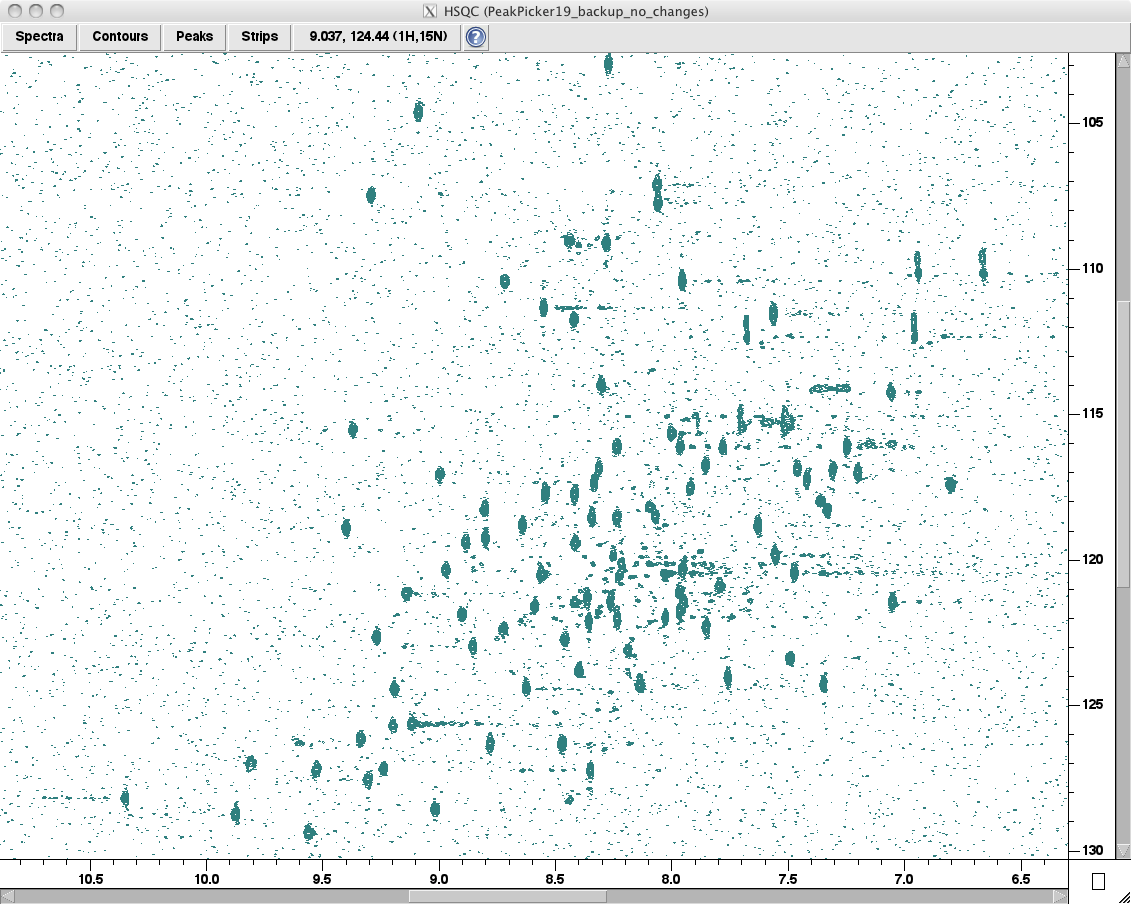
\includegraphics[scale=0.35]{figures/nhsqc}
  \caption[A frequency-domain NHSQC spectrum]
          {A frequency-domain NHSQC spectrum. 
           The x- and y-axes are nitrogen and proton, respectively.}
  \label{nhsqc}
\end{figure}

\begin{figure}
  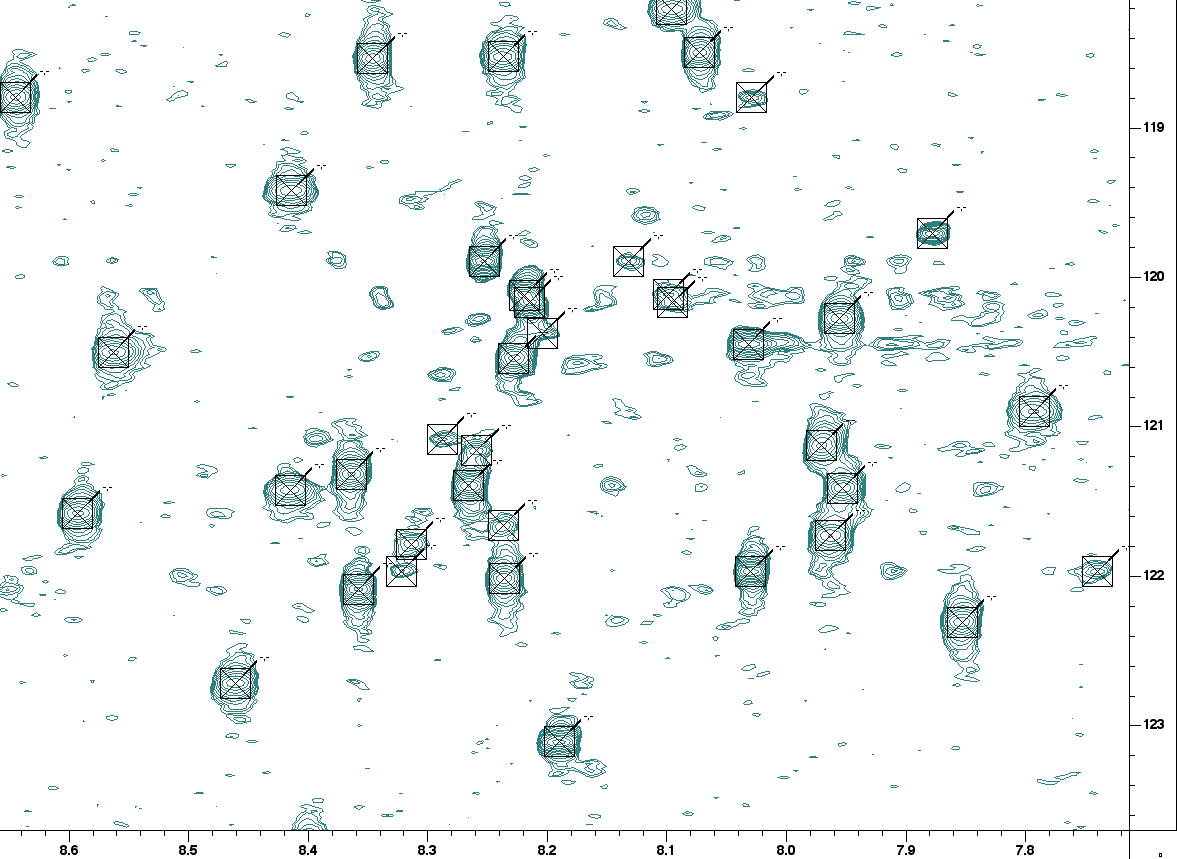
\includegraphics[scale=0.35]{figures/nhsqc_peaks}
  \caption[A peak-picked NHSQC spectrum]
          {A peak-picked NHSQC spectrum. 
           Peaks are indicated by black squares and crosses.}
  \label{nhsqc_peaks}
\end{figure}

\begin{figure}
  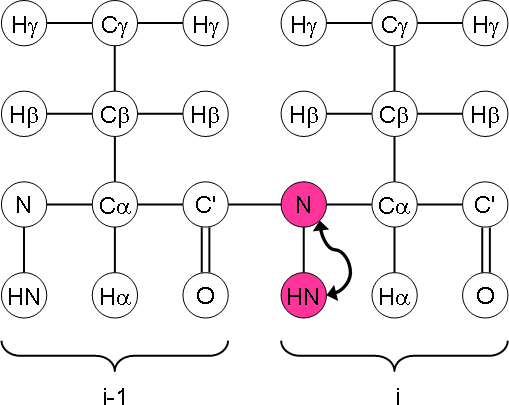
\includegraphics[scale=0.75]{figures/ccpn_nhsqc}
  \caption[The nuclei correlated by an NHSQC.]
          {The nuclei correlated (red) by an NHSQC.
           This figure is reproduced from \url{http://www.protein-nmr.org.uk/}
           with the permission of Victoria Higman.}
  \label{ccpn_nhsqc}
\end{figure}

\begin{figure}
  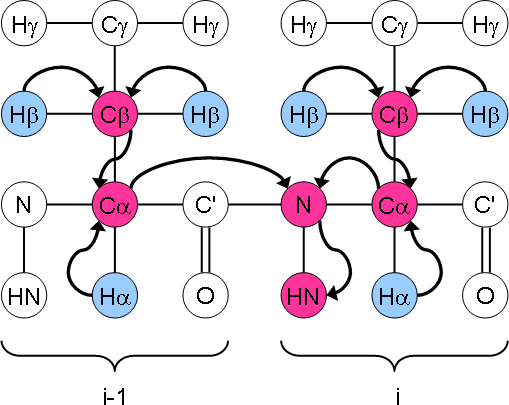
\includegraphics[scale=0.75]{figures/ccpn_hncacb}
  \caption[The nuclei correlated by an HNCACB.]
          {The nuclei correlated (red) by an HNCACB.
           This figure is reproduced from \url{http://www.protein-nmr.org.uk/}
           with the permission of Victoria Higman.}
  \label{ccpn_hncacb}
\end{figure}

\begin{figure}
  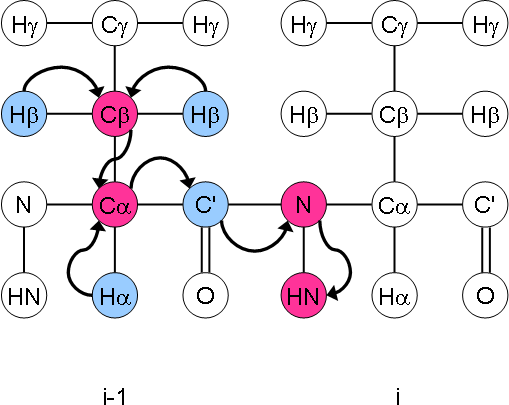
\includegraphics[scale=0.75]{figures/ccpn_cbcaconh}
  \caption[The nuclei correlated by a CBCA(CO)NH.]
          {The nuclei correlated (red) by a CBCA(CO)NH.
           This figure is reproduced from \url{http://www.protein-nmr.org.uk/}
           with the permission of Victoria Higman.}
  \label{ccpn_cbcaconh}
\end{figure}

\begin{figure}
  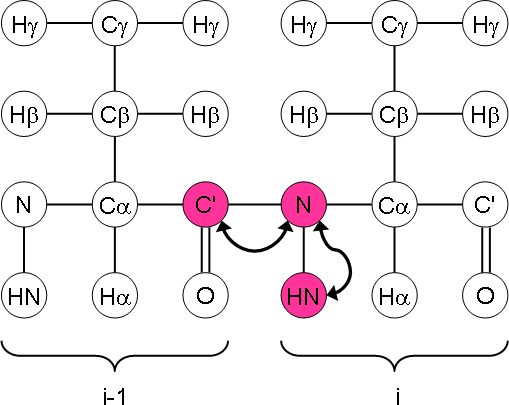
\includegraphics[scale=0.75]{figures/ccpn_hnco}
  \caption[The nuclei correlated by an HNCO.]
          {The nuclei correlated (red) by an HNCO.
           This figure is reproduced from \url{http://www.protein-nmr.org.uk/}
           with the permission of Victoria Higman.}
  \label{ccpn_hnco}
\end{figure}

\begin{figure}
  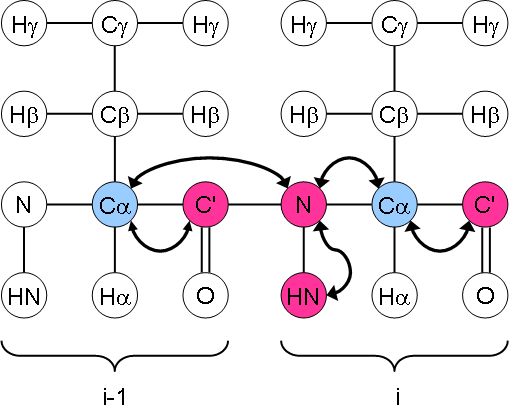
\includegraphics[scale=0.75]{figures/ccpn_hncaco}
  \caption[The nuclei correlated by an HN(CA)CO.]
          {The nuclei correlated (red) by an HN(CA)CO.
           This figure is reproduced from \url{http://www.protein-nmr.org.uk/}
           with the permission of Victoria Higman.}
  \label{ccpn_hncaco}
\end{figure}

\begin{figure}
  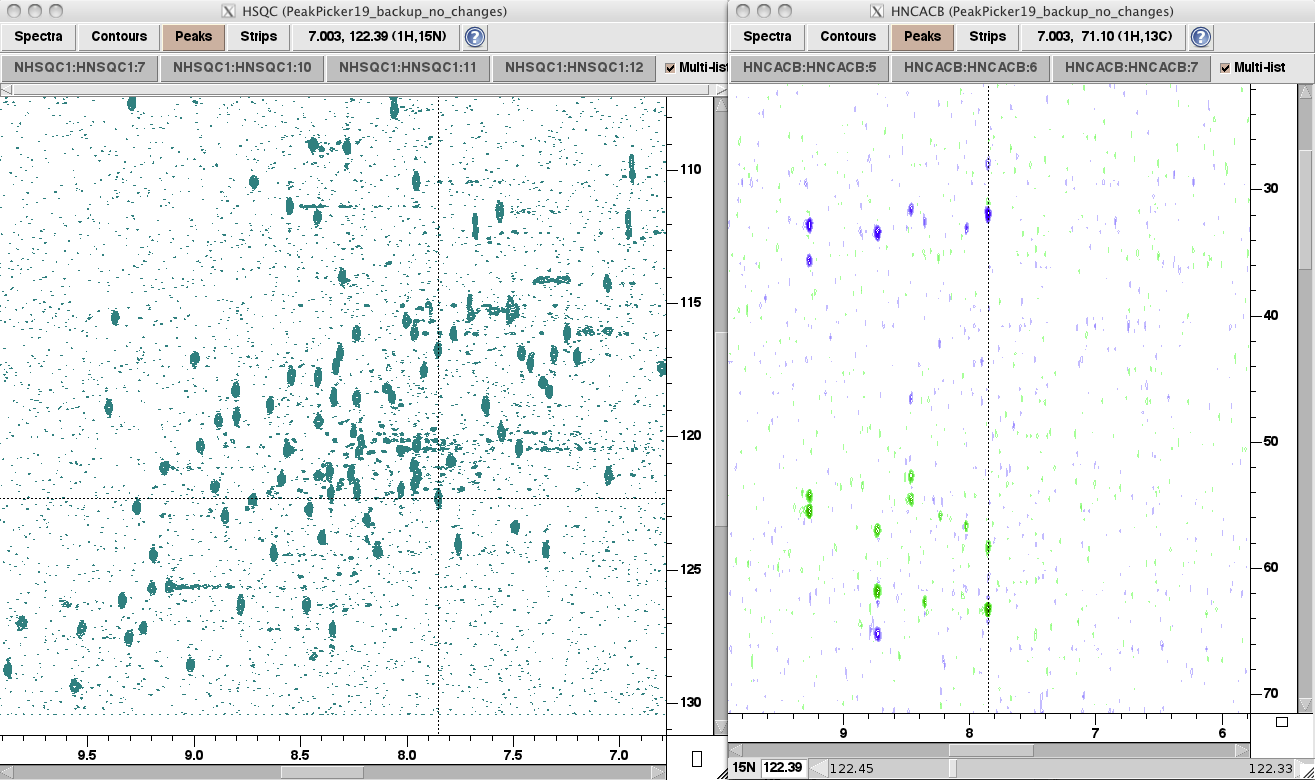
\includegraphics[scale=0.3]{figures/nhsqc_hncacb}
  \caption[Matching peaks between an NHSQC and an HNCACB spectrum]
          {Matching peaks between an NHSQC and an HNCACB spectrum.
           This likely indicates that the peaks belong to the same GSS.}
  \label{nhsqc_hncacb}
\end{figure}

\begin{figure}
  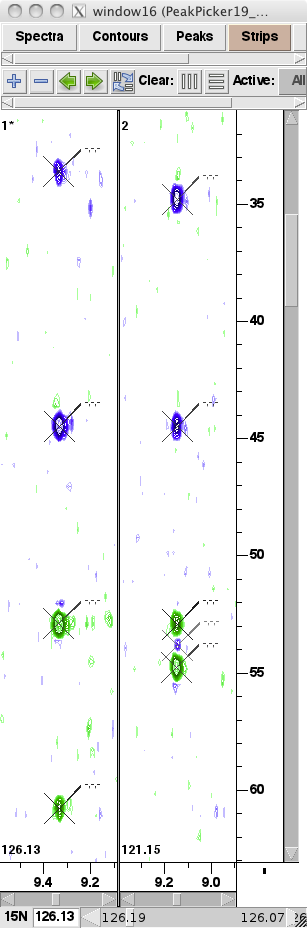
\includegraphics[scale=0.35]{figures/hncacb_overlap}
  \caption{Overlap of Carbon resonances in an HNCACB spectrum.}
  \label{hncacb_overlap}
\end{figure}

\begin{figure}
  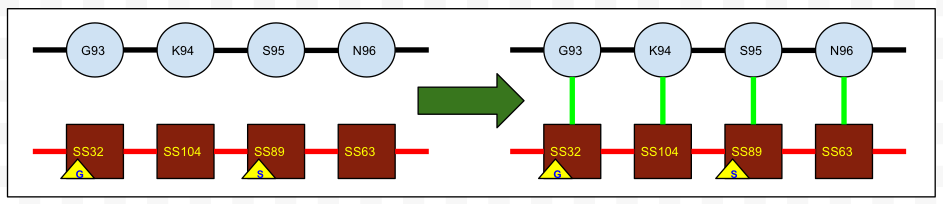
\includegraphics[scale=0.45]{figures/ss-residue}
  \caption[Assignment of a GSS chain to residues]
          {Assignment of a GSS chain to residues.  The circles are residues,
           black lines are peptide bonds, squares are GSSs, red lines are 
           sequential GSS assignments, and green lines are GSS-residue 
           assignments.}
  \label{ss-residue}
\end{figure}

\begin{figure}
  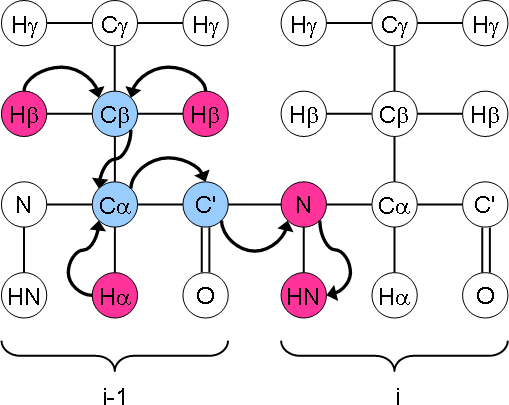
\includegraphics[scale=0.75]{figures/ccpn_hbhaconh}
  \caption[The nuclei correlated by an HBHA(CO)NH.]
          {The nuclei correlated (red) by an HBHA(CO)NH.
           This figure is reproduced from \url{http://www.protein-nmr.org.uk/}
           with the permission of Victoria Higman.}
  \label{ccpn_hbhaconh}
\end{figure}

\begin{figure}
  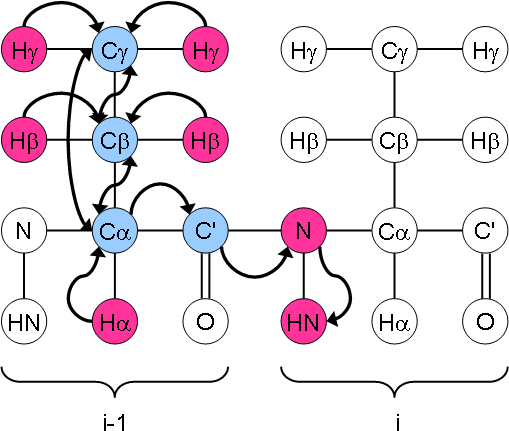
\includegraphics[scale=0.75]{figures/ccpn_hcconhtocsy}
  \caption[The nuclei correlated by an H(CCO)NH-Tocsy.]
          {The nuclei correlated (red) by an H(CCO)NH-Tocsy.
           This figure is reproduced from \url{http://www.protein-nmr.org.uk/}
           with the permission of Victoria Higman.}
  \label{ccpn_hcconhtocsy}
\end{figure}

\begin{figure}
  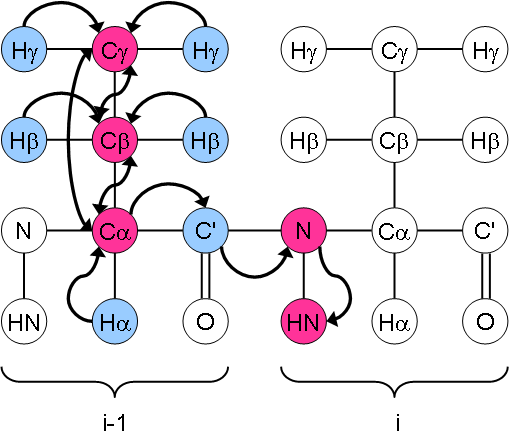
\includegraphics[scale=0.75]{figures/ccpn_cconhtocsy}
  \caption[The nuclei correlated by a C(CO)NH-Tocsy.]
          {The nuclei correlated (red) by a C(CO)NH-Tocsy.
           This figure is reproduced from \url{http://www.protein-nmr.org.uk/}
           with the permission of Victoria Higman.}
  \label{ccpn_cconhtocsy}
\end{figure}

\begin{figure}
  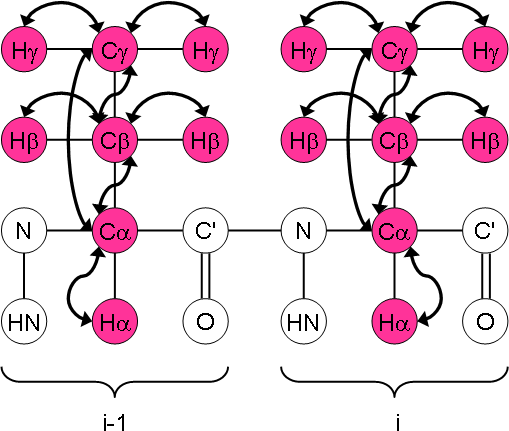
\includegraphics[scale=0.75]{figures/ccpn_hcchtocsy}
  \caption[The nuclei correlated by an HCCH-Tocsy.]
          {The nuclei correlated (red) by an HCCH-Tocsy.
           This figure is reproduced from \url{http://www.protein-nmr.org.uk/}
           with the permission of Victoria Higman.}
  \label{ccpn_hcchtocsy}
\end{figure}






% TODO appendices

% not sure what the difference is between `unsrt` and `ieeetr`
% also see `natbib` for another possible alternative
%\bibliographystyle{unsrt}
\bibliographystyle{ieeetr}
\bibliography{thesis}

\end{document}

